\documentclass{beamer}
\usepackage{physics}
\usepackage{amsmath}
\usepackage{tikz}
\usepackage{mathdots}
\usepackage{yhmath}
\usepackage{cancel}
\usepackage{color}
\usepackage{siunitx}
\usepackage{array}
\usepackage{multirow}
\usepackage{amssymb}
\usepackage{mathtools}
\usepackage{textcomp, gensymb}
\usepackage{tabularx}
\usepackage{extarrows}
\usepackage{booktabs}
\usetikzlibrary{fadings}
\usetikzlibrary{patterns}
\usetikzlibrary{shadows.blur}
\usetikzlibrary{shapes}
\usepackage[style=verbose,backend=bibtex]{biblatex}
\addbibresource{boltzmann.bib}
\usepackage{listings}
\usepackage{hyperref}

\newcommand{\pair}[1]{\langle #1 \rangle}
\DeclareMathOperator{\ee}{e}
\DeclareMathOperator{\ii}{i}
\DeclareMathOperator{\timeorder}{\mathcal{T}}

\newcommand{\concept}[1]{\textbf{#1}}

%region Theme
\usetheme{Madrid}

% Show section in foot
\makeatletter
\setbeamertemplate{footline}
{
  \leavevmode%
  \hbox{%
  \begin{beamercolorbox}[wd=.333333\paperwidth,ht=2.25ex,dp=1ex,center]{author in head/foot}%
    \usebeamerfont{author in head/foot}\insertauthor
  \end{beamercolorbox}%
  \begin{beamercolorbox}[wd=.333333\paperwidth,ht=2.25ex,dp=1ex,center]{title in head/foot}%
    \usebeamerfont{title in head/foot}\insertsection
  \end{beamercolorbox}%
  \begin{beamercolorbox}[wd=.333333\paperwidth,ht=2.25ex,dp=1ex,right]{date in head/foot}%
    \usebeamerfont{date in head/foot}\insertshortdate{}\hspace*{2em}
    \insertframenumber{} / \inserttotalframenumber\hspace*{2ex} 
  \end{beamercolorbox}}%
  \vskip0pt%
}
\makeatother

%endregion

%Information to be included in the title page:
\title{Time-dependent adiabatic $GW$}
\author{Jinyuan Wu}

\begin{document}

\maketitle

\begin{frame}
\frametitle{Table of content}

\tableofcontents    

\end{frame}

\section{Overview}

\section{Kadanoff-Baym equations}

\begin{frame}
\frametitle{Non-equilibrium Green function}

\textbf{Motivation} 

\begin{equation}
    \expval*{A} = \expval*{S^{-1} \timeorder_t ( S A_{\text{I}}(t) )}, \quad S = U(\infty, -\infty)
\end{equation}
Non-equilibrium state: not pure; contains excited state components;

$\ket*{\Psi_n}$ is excited state $\Rightarrow$ $S \ket*{\Psi_n} \neq \ee^{\ii \alpha} \ket*{\Psi_n}$
$\Rightarrow$ we can't peel the $S^{-1}$ off!!

\vspace{0.5cm}

\textbf{Solution} Four (instead of one) types of propagators: (note $S^{-1}$ is \emph{anti}-time ordered)

\begin{center}
    \small
    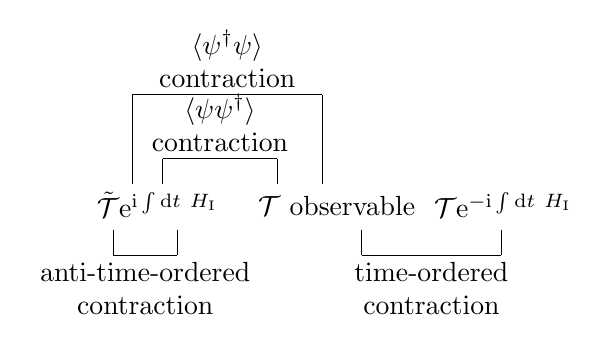
\begin{tikzpicture}[x=0.75pt,y=0.75pt,yscale=-0.7,xscale=0.7]
    %uncomment if require: \path (0,300); %set diagram left start at 0, and has height of 300
    
    %Straight Lines [id:da3326778841678064] 
    \draw    (135,167) -- (135,184.6) ;
    %Straight Lines [id:da14207491665960603] 
    \draw    (179,167) -- (179,184.6) ;
    %Straight Lines [id:da9585241583566635] 
    \draw    (135,184.6) -- (179,184.6) ;
    %Straight Lines [id:da5708657905713688] 
    \draw    (306,167) -- (306,184.6) ;
    %Straight Lines [id:da9177451110065487] 
    \draw    (402,167) -- (402,184.6) ;
    %Straight Lines [id:da6223566418192004] 
    \draw    (306,184.6) -- (402,184.6) ;
    %Straight Lines [id:da8688775028052254] 
    \draw    (169,118.4) -- (169,136) ;
    %Straight Lines [id:da16336389755134917] 
    \draw    (248,118.4) -- (248,136) ;
    %Straight Lines [id:da09889506498736633] 
    \draw    (169,118.4) -- (248,118.4) ;
    %Straight Lines [id:da5570498155343657] 
    \draw    (148,74.3) -- (148,136) ;
    %Straight Lines [id:da7392127913533113] 
    \draw    (148,74.3) -- (279,74.3) ;
    %Straight Lines [id:da826347580065202] 
    \draw    (279,74.3) -- (279,136) ;
    
    % Text Node
    \draw (122,139.5) node [anchor=north west][inner sep=0.75pt]    {$\tilde{\mathcal{T}} \mathrm{e}^{\mathrm{i}\int \mathrm{d} t\ H_{\text{I}}}$};
    % Text Node
    \draw (233,142) node [anchor=north west][inner sep=0.75pt]   [align=left] {$\displaystyle \mathcal{T}$ observable};
    % Text Node
    \draw (354,139.5) node [anchor=north west][inner sep=0.75pt]    {$\mathcal{T}\mathrm{e}^{-\mathrm{i}\int \mathrm{d} t\ H_{\text{I}}}$};
    % Text Node
    \draw (157,187.6) node [anchor=north] [inner sep=0.75pt]   [align=left] {\begin{minipage}[lt]{83.43pt}\setlength\topsep{0pt}
    \begin{center}
    anti-time-ordered \\contraction
    \end{center}
    
    \end{minipage}};
    % Text Node
    \draw (354,187.6) node [anchor=north] [inner sep=0.75pt]   [align=left] {\begin{minipage}[lt]{62.78pt}\setlength\topsep{0pt}
    \begin{center}
    time-ordered \\contraction
    \end{center}
    
    \end{minipage}};
    % Text Node
    \draw (208.5,115.4) node [anchor=south] [inner sep=0.75pt]   [align=left] {\begin{minipage}[lt]{52.85pt}\setlength\topsep{0pt}
    \begin{center}
    $\displaystyle \langle \psi \psi ^{\dagger } \rangle $\\contraction
    \end{center}
    
    \end{minipage}};
    % Text Node
    \draw (213.5,71.3) node [anchor=south] [inner sep=0.75pt]   [align=left] {\begin{minipage}[lt]{52.85pt}\setlength\topsep{0pt}
    \begin{center}
    $\displaystyle \langle \psi ^{\dagger } \psi \rangle $\\contraction
    \end{center}
    
    \end{minipage}};
    
    
    \end{tikzpicture}
        
\end{center}

\end{frame}

\begin{frame}
\frametitle{Keldysh formalism}

\textbf{Four types of (fermionic) propagators}

\begin{equation}
    \begin{aligned}
        \ii G^{--} &= \ii G^{\text{c}} = \expval*{\timeorder \psi_1 \psi_2^\dagger}, \quad 
        \ii G^{++} = \ii G^{\text{a}} = \expval*{\tilde{\timeorder} \psi_1 \psi_2^\dagger}, \\
        \ii G^{+-} &= \ii G^{>} = \expval*{\psi_1 \psi_2^\dagger},   \quad 
        \ii G^{-+} = \ii G^{<} = - \expval*{\psi_2^\dagger \psi_1}.
    \end{aligned}
\end{equation}    

\vspace{0.5cm}

\textbf{Diagrams} 

\begin{center}
    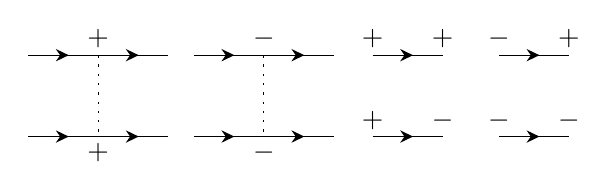
\begin{tikzpicture}[x=0.75pt,y=0.75pt,yscale=-0.7,xscale=0.7]
    %uncomment if require: \path (0,300); %set diagram left start at 0, and has height of 300
    
    %Straight Lines [id:da8169580565348766] 
    \draw    (35,78) -- (83.17,78) ;
    \draw [shift={(62.88,78)}, rotate = 180] [fill={rgb, 255:red, 0; green, 0; blue, 0 }  ][line width=0.08]  [draw opacity=0] (8.93,-4.29) -- (0,0) -- (8.93,4.29) -- (5.93,0) -- cycle    ;
    %Straight Lines [id:da9357207883622545] 
    \draw    (83.17,78) -- (131.33,78) ;
    \draw [shift={(111.05,78)}, rotate = 180] [fill={rgb, 255:red, 0; green, 0; blue, 0 }  ][line width=0.08]  [draw opacity=0] (8.93,-4.29) -- (0,0) -- (8.93,4.29) -- (5.93,0) -- cycle    ;
    %Straight Lines [id:da48155815853606776] 
    \draw    (35,134) -- (83.17,134) ;
    \draw [shift={(62.88,134)}, rotate = 180] [fill={rgb, 255:red, 0; green, 0; blue, 0 }  ][line width=0.08]  [draw opacity=0] (8.93,-4.29) -- (0,0) -- (8.93,4.29) -- (5.93,0) -- cycle    ;
    %Straight Lines [id:da7480670839969836] 
    \draw    (83.17,134) -- (131.33,134) ;
    \draw [shift={(111.05,134)}, rotate = 180] [fill={rgb, 255:red, 0; green, 0; blue, 0 }  ][line width=0.08]  [draw opacity=0] (8.93,-4.29) -- (0,0) -- (8.93,4.29) -- (5.93,0) -- cycle    ;
    %Straight Lines [id:da4153723089787493] 
    \draw  [dash pattern={on 0.84pt off 2.51pt}]  (83.17,78) -- (83.17,134) ;
    %Straight Lines [id:da9154821765962851] 
    \draw    (149,78) -- (197.17,78) ;
    \draw [shift={(176.88,78)}, rotate = 180] [fill={rgb, 255:red, 0; green, 0; blue, 0 }  ][line width=0.08]  [draw opacity=0] (8.93,-4.29) -- (0,0) -- (8.93,4.29) -- (5.93,0) -- cycle    ;
    %Straight Lines [id:da3027826223354886] 
    \draw    (197.17,78) -- (245.33,78) ;
    \draw [shift={(225.05,78)}, rotate = 180] [fill={rgb, 255:red, 0; green, 0; blue, 0 }  ][line width=0.08]  [draw opacity=0] (8.93,-4.29) -- (0,0) -- (8.93,4.29) -- (5.93,0) -- cycle    ;
    %Straight Lines [id:da1521558171041284] 
    \draw    (149,134) -- (197.17,134) ;
    \draw [shift={(176.88,134)}, rotate = 180] [fill={rgb, 255:red, 0; green, 0; blue, 0 }  ][line width=0.08]  [draw opacity=0] (8.93,-4.29) -- (0,0) -- (8.93,4.29) -- (5.93,0) -- cycle    ;
    %Straight Lines [id:da015084792241701894] 
    \draw    (197.17,134) -- (245.33,134) ;
    \draw [shift={(225.05,134)}, rotate = 180] [fill={rgb, 255:red, 0; green, 0; blue, 0 }  ][line width=0.08]  [draw opacity=0] (8.93,-4.29) -- (0,0) -- (8.93,4.29) -- (5.93,0) -- cycle    ;
    %Straight Lines [id:da8317921095867193] 
    \draw  [dash pattern={on 0.84pt off 2.51pt}]  (197.17,78) -- (197.17,134) ;
    %Straight Lines [id:da7041708770117445] 
    \draw    (272,78) -- (320.17,78) ;
    \draw [shift={(299.88,78)}, rotate = 180] [fill={rgb, 255:red, 0; green, 0; blue, 0 }  ][line width=0.08]  [draw opacity=0] (8.93,-4.29) -- (0,0) -- (8.93,4.29) -- (5.93,0) -- cycle    ;
    %Straight Lines [id:da24010158572243] 
    \draw    (272,134) -- (320.17,134) ;
    \draw [shift={(299.88,134)}, rotate = 180] [fill={rgb, 255:red, 0; green, 0; blue, 0 }  ][line width=0.08]  [draw opacity=0] (8.93,-4.29) -- (0,0) -- (8.93,4.29) -- (5.93,0) -- cycle    ;
    %Straight Lines [id:da3015830145357803] 
    \draw    (359,78) -- (407.17,78) ;
    \draw [shift={(386.88,78)}, rotate = 180] [fill={rgb, 255:red, 0; green, 0; blue, 0 }  ][line width=0.08]  [draw opacity=0] (8.93,-4.29) -- (0,0) -- (8.93,4.29) -- (5.93,0) -- cycle    ;
    %Straight Lines [id:da24391779212824316] 
    \draw    (359,134) -- (407.17,134) ;
    \draw [shift={(386.88,134)}, rotate = 180] [fill={rgb, 255:red, 0; green, 0; blue, 0 }  ][line width=0.08]  [draw opacity=0] (8.93,-4.29) -- (0,0) -- (8.93,4.29) -- (5.93,0) -- cycle    ;
    
    % Text Node
    \draw (83.17,75) node [anchor=south] [inner sep=0.75pt]   [align=left] {$+$};
    % Text Node
    \draw (83.17,137) node [anchor=north] [inner sep=0.75pt]   [align=left] {$+$};
    % Text Node
    \draw (197.17,75) node [anchor=south] [inner sep=0.75pt]   [align=left] {$-$};
    % Text Node
    \draw (197.17,137) node [anchor=north] [inner sep=0.75pt]   [align=left] {$-$};
    % Text Node
    \draw (272,75) node [anchor=south] [inner sep=0.75pt]   [align=left] {$+$};
    % Text Node
    \draw (320.17,75) node [anchor=south] [inner sep=0.75pt]   [align=left] {$+$};
    % Text Node
    \draw (272,131) node [anchor=south] [inner sep=0.75pt]   [align=left] {$+$};
    % Text Node
    \draw (320.17,131) node [anchor=south] [inner sep=0.75pt]   [align=left] {$-$};
    % Text Node
    \draw (359,75) node [anchor=south] [inner sep=0.75pt]   [align=left] {$-$};
    % Text Node
    \draw (407.17,75) node [anchor=south] [inner sep=0.75pt]   [align=left] {$+$};
    % Text Node
    \draw (359,131) node [anchor=south] [inner sep=0.75pt]   [align=left] {$-$};
    % Text Node
    \draw (407.17,131) node [anchor=south] [inner sep=0.75pt]   [align=left] {$-$};
    
    
    \end{tikzpicture}
    
\end{center}

\textbf{Self-energy} 

\begin{equation}
    G = \pmqty{
        G^{--} & G^{-+} \\ 
        G^{+-} & G^{++}
    }   , \quad 
    \Sigma = \pmqty{
        \Sigma^{--} & \Sigma^{-+} \\ 
        \Sigma^{+-} & \Sigma^{++}
    } , \quad 
    G = G_0 + G_0 \Sigma G.
\end{equation}

\end{frame}

\begin{frame}
\frametitle{Alternative formulation: Keldysh contour}

\textbf{Keldysh contour} The information in the $G$ matrix can be alternatively stored 
in a time-ordered Green function on \emph{Keldysh contour}

\begin{center}
    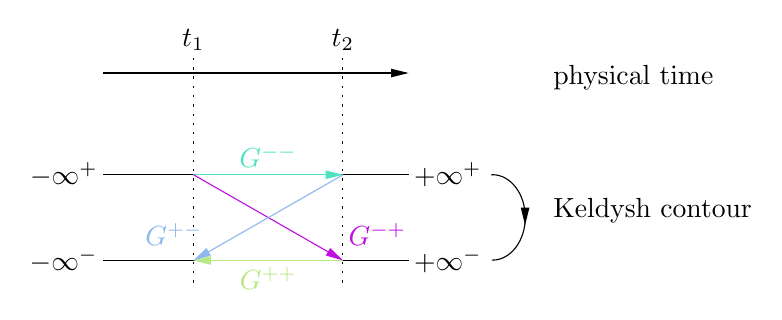
\begin{tikzpicture}[x=0.75pt,y=0.75pt,yscale=-0.7,xscale=0.7]
    %uncomment if require: \path (0,300); %set diagram left start at 0, and has height of 300
    
    %Straight Lines [id:da9923247639127166] 
    \draw    (144,152) -- (354.17,152) ;
    %Straight Lines [id:da5829772718809481] 
    \draw    (144,211) -- (354.17,211) ;
    %Straight Lines [id:da04548734740797422] 
    \draw  [dash pattern={on 0.84pt off 2.51pt}]  (206,71.6) -- (206,229) ;
    %Straight Lines [id:da1610984974972618] 
    \draw  [dash pattern={on 0.84pt off 2.51pt}]  (309,71.6) -- (309,229) ;
    %Straight Lines [id:da04350669910867855] 
    \draw    (144,82) -- (352.17,82) ;
    \draw [shift={(354.17,82)}, rotate = 180] [fill={rgb, 255:red, 0; green, 0; blue, 0 }  ][line width=0.08]  [draw opacity=0] (12,-3) -- (0,0) -- (12,3) -- cycle    ;
    %Straight Lines [id:da9269008755131121] 
    \draw [color={rgb, 255:red, 80; green, 227; blue, 194 }  ,draw opacity=1 ]   (206.17,152) -- (307.17,152) ;
    \draw [shift={(309.17,152)}, rotate = 180] [fill={rgb, 255:red, 80; green, 227; blue, 194 }  ,fill opacity=1 ][line width=0.08]  [draw opacity=0] (12,-3) -- (0,0) -- (12,3) -- cycle    ;
    %Straight Lines [id:da9541927407052295] 
    \draw [color={rgb, 255:red, 184; green, 233; blue, 134 }  ,draw opacity=1 ]   (208.17,211) -- (309.17,211) ;
    \draw [shift={(206.17,211)}, rotate = 0] [fill={rgb, 255:red, 184; green, 233; blue, 134 }  ,fill opacity=1 ][line width=0.08]  [draw opacity=0] (12,-3) -- (0,0) -- (12,3) -- cycle    ;
    %Straight Lines [id:da8455403205757837] 
    \draw [color={rgb, 255:red, 189; green, 16; blue, 224 }  ,draw opacity=1 ]   (206.17,152) -- (307.43,210.01) ;
    \draw [shift={(309.17,211)}, rotate = 209.8] [fill={rgb, 255:red, 189; green, 16; blue, 224 }  ,fill opacity=1 ][line width=0.08]  [draw opacity=0] (12,-3) -- (0,0) -- (12,3) -- cycle    ;
    %Straight Lines [id:da6613881717892212] 
    \draw [color={rgb, 255:red, 141; green, 183; blue, 237 }  ,draw opacity=1 ]   (309.17,152) -- (207.9,210.01) ;
    \draw [shift={(206.17,211)}, rotate = 330.2] [fill={rgb, 255:red, 141; green, 183; blue, 237 }  ,fill opacity=1 ][line width=0.08]  [draw opacity=0] (12,-3) -- (0,0) -- (12,3) -- cycle    ;
    %Shape: Arc [id:dp9263560588014466] 
    \draw  [draw opacity=0] (411.17,152) .. controls (411.43,151.99) and (411.69,151.98) .. (411.95,151.98) .. controls (424.42,151.98) and (434.53,165.14) .. (434.53,181.37) .. controls (434.53,197.6) and (424.42,210.76) .. (411.95,210.76) .. controls (411.84,210.76) and (411.73,210.76) .. (411.62,210.76) -- (411.95,181.37) -- cycle ; \draw   (411.17,152) .. controls (411.43,151.99) and (411.69,151.98) .. (411.95,151.98) .. controls (424.42,151.98) and (434.53,165.14) .. (434.53,181.37) .. controls (434.53,197.6) and (424.42,210.76) .. (411.95,210.76) .. controls (411.84,210.76) and (411.73,210.76) .. (411.62,210.76) ;  
    %Straight Lines [id:da9478596817855973] 
    \draw    (434.42,181.77) -- (434.42,184.6) ;
    \draw [shift={(434.42,186.6)}, rotate = 270] [fill={rgb, 255:red, 0; green, 0; blue, 0 }  ][line width=0.08]  [draw opacity=0] (12,-3) -- (0,0) -- (12,3) -- cycle    ;
    
    % Text Node
    \draw (142,152) node [anchor=east] [inner sep=0.75pt]    {$-\infty ^{+}$};
    % Text Node
    \draw (142,211) node [anchor=east] [inner sep=0.75pt]    {$-\infty ^{-}$};
    % Text Node
    \draw (356.17,152) node [anchor=west] [inner sep=0.75pt]    {$+\infty ^{+}$};
    % Text Node
    \draw (356.17,211) node [anchor=west] [inner sep=0.75pt]    {$+\infty ^{-}$};
    % Text Node
    \draw (452,176.5) node [anchor=west] [inner sep=0.75pt]   [align=left] {Keldysh contour};
    % Text Node
    \draw (206,68.6) node [anchor=south] [inner sep=0.75pt]    {$t_{1}$};
    % Text Node
    \draw (309,68.6) node [anchor=south] [inner sep=0.75pt]    {$t_{2}$};
    % Text Node
    \draw (257.67,149) node [anchor=south] [inner sep=0.75pt]  [color={rgb, 255:red, 80; green, 227; blue, 194 }  ,opacity=1 ]  {$G^{--}$};
    % Text Node
    \draw (257.67,214) node [anchor=north] [inner sep=0.75pt]  [color={rgb, 255:red, 184; green, 233; blue, 134 }  ,opacity=1 ]  {$G^{++}$};
    % Text Node
    \draw (171.17,202.39) node [anchor=south west] [inner sep=0.75pt]  [color={rgb, 255:red, 141; green, 183; blue, 237 }  ,opacity=1 ]  {$G^{+-}$};
    % Text Node
    \draw (311.17,202.39) node [anchor=south west] [inner sep=0.75pt]  [color={rgb, 255:red, 189; green, 16; blue, 224 }  ,opacity=1 ]  {$G^{-+}$};
    % Text Node
    \draw (452,85.17) node [anchor=west] [inner sep=0.75pt]   [align=left] {physical time};
    
    
    \end{tikzpicture}
    
\end{center}


\end{frame}

\begin{frame}
\frametitle{Green function EOM}

\textbf{From Keldysh contour to physical contour} Lengreth theorem: 

\begin{equation}
    \begin{aligned}
        (AB)^< &= A^{\text{R}} B^< + A^< B^{\text{A}}, \quad 
        (AB)^> = A^{\text{R}} B^> + A^> B^{\text{A}}, \quad \\
        (AB)^{\text{R}} &= A^{\text{R}} B^{\text{R}}, \quad 
        (AB)^{\text{A}} = A^{\text{A}} B^{\text{A}},
    \end{aligned}
\end{equation}
where
\begin{equation}
    \begin{aligned}
        &A^>(t_1, t_2) = A(t_1^+, t_2^-), \quad 
        A^<(t_1, t_2) = A(t_1^-, t_2^+), \quad \\
        &A^{\text{R}}(t_1, t_2) = \theta(t_1 - t_2) (A^> - A^<).
    \end{aligned}
\end{equation}

Mapping an equation on Keldysh contour to its counterpart on the physical time axis!


\end{frame}


\begin{frame}[allowframebreaks]
\frametitle{Derivation of EOM of $G^{<,>}$ and $G^{\text{A}}$}

\textbf{Recommended references} The following series:
\begin{itemize}
    \item \cite{vspivcka2005long} 
    \item \cite{rammer1986quantum}
\end{itemize}

\vspace{0.25cm}

\framebreak

\textbf{From self-energy correction to EOM} From Lengreth theorem:
\begin{equation}
    G = G_0 + G_0 \Sigma G \Rightarrow 
    G^< = G^<_0 + G^<_0 \Sigma^{\text{A}} G^{\text{A}}
    + G_0^{\text{R}} \Sigma^{\text{R}} G^< 
    + G_0^{\text{R}} \Sigma^{<} G^\text{A} ,
    \label{eq:lesser-eom-1}
\end{equation}
\begin{equation}
    G = G_0 + G \Sigma G_0 \Rightarrow 
    G^< = G^<_0 + G^{\text{R}}_0 \Sigma^{\text{R}} G^{<}_0
    + G^{\text{R}} \Sigma^{<} G^{\text{A}}_0 
    + G^{<} \Sigma^{\text{A}} G^\text{A} ,
    \label{eq:lesser-eom-2}
\end{equation}
\begin{equation}
    G^{\text{A}} = G^{\text{A}}_0 + G^{\text{A}}_0 \Sigma^{\text{A}} G^{\text{A}}, \quad 
    G^{\text{R}} = G^{\text{R}}_0 + G^{\text{R}}_0 \Sigma^{\text{R}} G^{\text{R}}.
    \label{eq:G-a-r-eom-original}
\end{equation}

\vspace{0.25cm}

\textbf{Getting rid of $G_0$} We define 
\begin{equation}
    G_0^{-1} \coloneqq \ii \partial_t - H_0,
\end{equation}
and 
\begin{equation}
    G_0^{-1} G_0^{\text{A}, \text{R}} = I, \quad 
    G_0^{-1} G_0^{<,>} = 0.
\end{equation}
Taking complex conjugate of the def. of $G^{<,>}_0$ we find 
(left arrow = apply $\partial_t$ and $H_0$ to the second index of $G_0^{<,>}$)
\begin{equation}
    G_0^{<,>} (- \ii \overleftarrow{\partial_{t_2}} - H_0) = 0.
\end{equation}

\framebreak

\textbf{The Schr\"{o}dinger-like EOM} Applying $G_0^{-1}$
to the left of \eqref{eq:lesser-eom-1} and to the right of \eqref{eq:lesser-eom-2}:
\begin{equation}
    (\ii \partial_{t_1} - H_0) G^<(1,2) = \Sigma^{\text{R}} G^< + \Sigma^< G^{\text{A}},
\end{equation}
\begin{equation}
    - \ii \partial_{t_2} G^<(1, 2) - G^< H_0 = G^{\text{R}} \Sigma^< + G^< \Sigma^{\text{A}},
\end{equation}
\begin{equation}
    \Rightarrow \ii (\partial_{t_1} + \partial_{t_2}) G^< - \comm*{H_0}{G^<} = 
    \Sigma^{\text{R}} G^< + \Sigma^< G^{\text{A}} - G^{\text{R}} \Sigma^< - G^< \Sigma^{\text{A}}.
\end{equation}

\vspace{0.25cm}

\textbf{Mixed coordinates} We define ``average time'' and ``relative time'':
\begin{equation}
    T = \frac{t_1 + t_2}{2}, \quad t = t_1 - t_2,
\end{equation}
\begin{equation}
    \Rightarrow \pdv{T} = \pdv{t_1} + \pdv{t_2}.
\end{equation}
We then do Fourier transform over $t$: 
similar to the equilibrium case. 
($T$ $\simeq$ driving, $t$ $\simeq$ internal time evolution)


\end{frame}



\section{Quantum master equation}

\begin{frame}
    \frametitle{Towards a single-time formalism}
    
    \textbf{Summary up to now} \begin{itemize}
        \item \emph{Accurate} EOMs about $G^{\text{A}, \text{R}}$, and EOM of $G^<$: 
        \begin{equation}
            \ii \partial_T G^< - \comm*{H_0}{G^<} = 
            \Sigma^{\text{R}} G^< + \Sigma^< G^{\text{A}} - G^{\text{R}} \Sigma^< - G^< \Sigma^{\text{A}}.
        \end{equation}
        The RHS contains $t$ (or $\omega$) and $G^<$.
        \item Note: we can actually put the $t=0$ part of $\Sigma$ into $H_0$!
            $\Rightarrow$ Example: COHSEX TD-aGW
    \end{itemize}

    \vspace{0.25cm}

    \textbf{Goal} Obtaining quantum kinetics: 
    \begin{itemize}
        \item Quantum master equation (QME), i.e. EOM of $\rho(\vb*{r}_1, \vb*{r}_2, t)$,
        \item and its long wave length limit, the quantum Boltzmann equation (QBE)
    \end{itemize} 
    
    \vspace{0.25cm}

    \textbf{Problem} Both LHS and RHS contain $\omega$: problem too large. 

    \textbf{What we want} Obtaining a close form EOM about $G^<(T, t=0)$

\end{frame}

\begin{frame}
    \frametitle{Quantum master equation}
    
    \textbf{Reduced density  matrix} Single-electron density matrix:
    \begin{equation}
        \ii \rho(T) = G^<(T, t = 0) = \int \frac{\dd{\omega}}{2\pi}  G^<(T, \omega)
    \end{equation}
    
    \vspace{0.25cm}

    \textbf{What we want} Two types of reduction:
    \begin{itemize}
        \item Reducing $\Sigma$ to an easy function of $G$, ideally $G^<$
        \item Reducing $G^<$ to $\rho(T)$
    \end{itemize} 
    
    \vspace{0.25cm}

    \textbf{Reducing $\Sigma$} \begin{itemize}
        \item Always possible: we can formally eliminate $\chi, \epsilon$, etc. from Hedin eq. 
            and get a $\Sigma$ about $G$ i.e. about $G^<, G^{\text{A}, \text{R}}$
        \item But then $G^{\text{A}, \text{B}}$ can be eliminated with \eqref{eq:G-a-r-eom-original} as well
        \item In reality: a truncation is needed \dots
    \end{itemize}

\end{frame}

\begin{frame}
\frametitle{Reconstruction of $G^<$ from $\rho$}

\textbf{Reconstruction theorem} From $\rho$, $G^{\text{A}, \text{R}}$
(which can be calculated using \eqref{eq:G-a-r-eom-original} from $\rho$),
$G^<$ can be completely restored\footcite{vspivcka2005long} 

\vspace{0.25cm} 

\textbf{Constructive proof} See (71) in the reference;
note that 
\begin{equation}
    \begin{aligned}
        (G^{\text{R}})^{-1} \theta(t_1 - t_2) G^< &= 
        (\partial_{t_1} - H_0 - \Sigma^{\text{R}}) \theta(t_1 - t_2) G^< \\
        &= \delta(t_1 - t_2) G^< 
        + \theta(t_1 - t_2) (\partial_{t_1} - H_0 - \Sigma^{\text{R}}) G^< \\
        &= \rho(t_1) + \cdots
    \end{aligned}
\end{equation}

\end{frame}

\begin{frame}
\frametitle{Quantum master equation as an accurate formalism}

\textbf{Existence of accurate quantum master equation} 
In conclusion, in principle we can always write down something accurate like this:
\begin{equation}
    \pdv{\rho}{t} + \ii \comm*{H_0}{\rho} = \int_{-\infty}^{t} F[\rho(t')] \dd{t'},
\end{equation}
where $F$ is obtained from $\Sigma^{\text{R}} G^< + \Sigma^< G^{\text{A}} - G^{\text{R}} \Sigma^< - G^< \Sigma^{\text{A}}$,
and $G^{\text{R}, \text{A}}$ is reconstructed from $\rho$ 
by doing a complete self-energy run,
and $G^<$ is reconstructed from $G^\text{A}$ and $G^{\text{R}}$ and $\rho$.

\vspace{0.25pt}

\textbf{\dots but of course simplification is needed} 

\end{frame}

\begin{frame}
\frametitle{Gradient expansion: first step from QME to QBE}

\textbf{Mixed coordinates}
\begin{equation}
    \tilde{\rho}(\vb*{k}, \vb*{r}, t) = \int \dd{x} 
    \ee^{- \ii \vb*{k} \cdot \vb*{r}} \rho\left(
        \vb*{r} + \frac{\vb*{x}}{2}, \vb*{r} - \frac{\vb*{x}}{2}, t
    \right),
\end{equation}    
\begin{equation}
    \frac{1}{\ii} \widetilde{\comm*{H_0}{\rho}} = 
    \pdv{\epsilon}{\vb*{p}} \cdot \pdv{\tilde{\rho}}{\vb*{r}}
    - \pdv{\epsilon}{\vb*{r}} \cdot \pdv{\tilde{\rho}}{\vb*{p}} + \cdots
\end{equation}

\vspace{0.25cm}

\textbf{Gradient expansion} Only take the first two terms:
assuming no higher dependence

\end{frame}

\begin{frame}
\frametitle{Issue: the def. of $G_0$ and $\Sigma$}

\textbf{Ambiguity in the meaning of $\Sigma$}
\begin{itemize}
    \item In ordinary usage: $G_0$ directly from $H_0$
    \item But some prefer to move a part of $\Sigma$
        that looks like ``effective potential'' into $H_0$ \dots
    \item Thus: $G_0$ contains ``interactively corrected band structure'';
        $\Sigma$ contains ``scattering''??
\end{itemize}    

\vspace{0.25cm}

\textbf{Comparison with similar issue in QBE} \begin{itemize}
    \item When impurities are rare: they appear in collision integral
    \item When impurities are abundant: they lead to an impurity band \dots
        and appear in the diffusion term?
\end{itemize}

\vspace{0.25cm}

\textbf{Lacking proof of equivalence} \begin{itemize}
    \item Do different division of labor between $\Sigma$ and $G_0$
        lead to consistent results?
\end{itemize}

\end{frame}

\section{Quantum Boltzmann equation}

\begin{frame}
\frametitle{A radical move: quantum Boltzmann equation}

\textbf{Approximations leading to QBE} \begin{itemize}
    \item Gradient expansion: smooth $U_{\text{ext}}$:
    \begin{equation}
        \comm*{H_0}{\rho} 
    \end{equation}
    \item Quasiparticle approx.
    \begin{equation}
        G^<(\vb*{x}, \vb*{p}, T, \omega) = 2 \pi \delta(\omega - )
    \end{equation}
    Immediate problem: 
\end{itemize}    

TODO: how to get the Fermi golden rule??? 

\end{frame}

\section{What does TD-aGW see?}

\begin{frame}
    \frametitle{Example: TODO}

    

\end{frame}

\end{document}